%%%%%%%%%%%%%%%%%%%%%%%%%%%%%%%%%%%%%%%%%%%%%%%%%%%%%%%%
%%
\clearpage
\newpage
\section{The cal\_BADPIX recipe}
\label{ch:the_recipes:cal_BADPIX_spirou}
%%
%%%%%%%%%%%%%%%%%%%%%%%%%%%%%%%%%%%%%%%%%%%%%%%%%%%%%%%%

Recipe to generate the bad pixel map. \\

% -------------------------------------------------------
\subsection{The inputs}
% -------------------------------------------------------
The input of \calbadpix is as follows:
\begin{cmdbox}
cal_BADPIX_spirou.py  night_repository  flatfile, darkfile
\end{cmdbox}
\noindent or
\begin{pythonbox}
import cal_DARK_spirou
night_reposityory = '20170710'
darkfile = 'dark_dark02d406.fits'
flatfile = 'flat_flat02f10.fits'
cal_DARK_spirou.main(night_repository, flatfile=flatfile, darkfile=darkfile)
\end{pythonbox}

\noindent where `night\_repository' defines \argnightname and `filenames' define the list of files in \argfilenames. All files in filenames must be valid python strings separated by a space (command line) or in a line (python) and must have the folowing prefixes:
\noindent File prefixes allowed:
\begin{itemize}
	\item flat\_flat (flatfile)
	\item dark\_dark (darkfile)
\end{itemize}

% % -------------------------------------------------------
% \subsection{The outputs}
% % -------------------------------------------------------

% The outputs of \definevariable{text:badpixelfits}{badpixelfits} are as follows:

% \begin{itemize}
% \item {badpixelfits} in form:
% \begin{tcustomdir}
% \{\reduceddir\}\{date prefix\}\_\{file\}\_badpixelfits.fits
% \end{tcustomdir}
% \end{itemize}

% \noindent where `date prefix' is constructed from \argnightname and the file name is the first file in \argfilenames.

% % -------------------------------------------------------
% \subsection{Summary of procedure}
% % -------------------------------------------------------
% \begin{enumerate}
% \item {}
% \end{enumerate}


% % -------------------------------------------------------
% \subsection{Quality Control}
% % -------------------------------------------------------

% There are currently three quality control checks for cal\_DARK\_spirou
% \begin{itemize}
% \item Unexpected {} if: 
% 	\begin{equation}
	
% 	\end{equation}

% \end{itemize}

% If none of these quality control criteria are valid then the output file is passed into the \calibdb with key `{}'.


% % -------------------------------------------------------
% \newpage
% \subsection{Example working run}
% % -------------------------------------------------------

% An example run where everything worked is below:

% \begin{cmdboxprintspecial}
% @g

% @g
% \end{cmdboxprintspecial}


% % -------------------------------------------------------
% \newpage
% \subsection{Interactive mode}
% % -------------------------------------------------------


% \noindent In interactive mode (\definevariable{text:drs_plot}{DRS\_PLOT} = 1) three figures will also appear (see Figure \ref{figure:}).


% \begin{figure}

% \begin{center}
% \begin{minipage}{.495\textwidth}
% \begin{center}
% \includegraphics[width=\textwidth]{Figures/cal_DARK_spirou_1.pdf}
% a
% \end{center}
% \end{minipage}%
% \begin{minipage}{.495\textwidth}
% \begin{center}
% \includegraphics[width=\textwidth]{Figures/cal_DARK_spirou_2.pdf}
% b
% \end{center}
% \end{minipage}%
% \end{center}

% \begin{center}
% \begin{minipage}{.495\textwidth}
% \begin{center}
% \includegraphics[width=\textwidth]{Figures/cal_DARK_spirou_3.pdf}
% c
% \end{center}
% \end{minipage}%
% \end{center}

% \caption{\textbf{(a)} The image with overplot red and blue regions (red/blue rectangles). \textbf{(b)} The bad pixel mask, bad pixels have a value=1 (in black) and good pixels have a value=0 (in white). \textbf{(c)} Histograms of the image regions, the full image (in green), the blue section (in blue) and the red section (in red). \label{figure:cal_DARK_spirou}}
% \end{figure}